%% =====================================================================
%% Documento de Planejamento do Projeto — Entrega 01 (29/08/2026)
%% Experiência Criativa: Projeto Transformador II — BCC / PUCPR
%% Autora: Gabriela Sofia
%% Formatação: IEEEtran conference (padrão do template dos professores)
%% Compilar: pdflatex main && pdflatex main
%% =====================================================================
\documentclass[conference]{IEEEtran}
\IEEEoverridecommandlockouts

\usepackage[T1]{fontenc}
\usepackage[utf8]{inputenc}
\usepackage[brazil]{babel}
\usepackage{graphicx}
\usepackage{booktabs}
\usepackage{array}
\usepackage{amsmath,amssymb}
\usepackage{xcolor}
\usepackage{tikz}
\usetikzlibrary{arrows.meta,positioning,fit,backgrounds,shapes.misc}
\usepackage{cite}
\usepackage{url}
\usepackage[hidelinks]{hyperref}

% cores do diagrama
\definecolor{cAzul}{HTML}{1F4E79}
\definecolor{cVerm}{HTML}{C0504D}
\definecolor{cVerd}{HTML}{3F6F4A}
\definecolor{cCinz}{HTML}{7F7F7F}
\definecolor{cFundo}{HTML}{EEF3F8}
\definecolor{cFundoAux}{HTML}{F7F0EE}
\definecolor{cFundoPrd}{HTML}{EDF3EE}

\begin{document}

\title{Do corpus auditável à inferência causal: suscetibilidade urbana
a enchentes com modelo interpretável e camada de explicação}

\author{\IEEEauthorblockN{Gabriela Sofia}
\IEEEauthorblockA{Experiência Criativa: Projeto Transformador II\\
Bacharelado em Ciência da Computação --- PUCPR\\
Turma \textcolor{red}{7A} --- Equipe \textcolor{red}{N}\\
\{\texttt{gabriela.milani}\}@pucpr.edu.br}}

\maketitle

% =====================================================================
\section{Descrição do Projeto}

Enchentes urbanas não atingem apenas uma área delimitada em um mapa: elas
interrompem deslocamentos, pressionam sistemas de drenagem e expõem de forma mais
severa populações que já vivem em territórios com infraestrutura
insuficiente~\cite{tellman2021}. A leitura física do fenômeno se apoia em dois
descritores consolidados --- a posição vertical relativa à drenagem mais próxima,
medida pelo HAND~\cite{renno2008}, e o índice topográfico de
umidade~\cite{beven1979}, ambos derivados por fluxo D-infinity --- que a
literatura combina com inventários de ocorrência em modelos de aprendizado de
máquina.

O projeto não começa neste documento, e este plano só se entende a partir do que
a primeira entrega construiu. Ela montou a cadeia de evidência em ordem
deliberada: leitura territorial do problema, conversão em heurísticas e conjuntos
tabulares, recorte em \emph{patches} Sentinel, agregação de evidências externas
por região, formalização de manifests, \emph{registries} e QA, criação do
Protocolo C --- quatro portões documentais e quatro decisões de uso --- como
filtro de promoção de evidência e, só ao final, \emph{embeddings} DINOv2 sob
encoder congelado. O peso é conferível: 59 \emph{patches}, 128 ativos Sentinel,
36 conjuntos públicos, 87 manifests, 43 testes e 9 eventos candidatos. Aquela
entrega também declarou o próprio teto: sem negativo formal, treino
supervisionado permanece bloqueado.

O achado que orienta este plano veio de um teste de ablação daquela entrega. A
acurácia balanceada foi de 0,8855 com as variáveis heurísticas, 0,4834 ao
removê-las e 0,4689 no cenário \emph{image-only}: o classificador reconstruía
critérios do próprio projeto, não uma referência independente. O problema central
desta entrega decorre desse número. Trata-se de converter a cadeia de evidência
em inferência causal defensável, o que exige três condições juntas: nenhuma
variável derivada do rótulo como preditor; um negativo que seja ausência
observada e não ausência de registro, problema descrito como
\emph{positive-unlabeled} com controles contaminados~\cite{li2022pul} e agravado
por sub-reporte espacialmente correlacionado~\cite{agostini2024}; e validação
prospectiva, porque validação embaralhada mede interpolação.

Os objetivos são: derivar variáveis de terreno e chuva reprodutíveis, sem
nenhuma derivada do rótulo; constituir um conjunto de treino com
negativo observado; estimar um modelo interpretável e submetê-lo a validação
prospectiva, reportando o resultado mesmo quando negativo; e entregar esse modelo
como produto auditável. \textbf{Pergunta de pesquisa}: um modelo de
suscetibilidade construído somente sobre variáveis físico-hidrológicas
interpretáveis, treinado com eventos registrados e negativo observado, preserva
capacidade discriminativa sob validação prospectiva --- e é possível entregá-lo
como produto sem que a camada de linguagem natural altere, complete ou substitua
a decisão estatística?

A abordagem tem duas frentes: a causal estima o modelo sobre variáveis derivadas
de terreno e reanálise; a de produto o expõe por um contrato de inferência com
\emph{gates} obrigatórios, sobre o qual atua uma camada de explicação que
descreve o resultado e nunca o decide (Fig.~\ref{fig:pipeline}). Por ser um
plano, cada etapa da Seção~\ref{sec:etapas} declara a evidência que a encerra e a
rota alternativa caso ela não apareça.

% ------------------------------ FIGURA 1 ------------------------------
\begin{figure*}[!t]
\centering
\resizebox{0.64\textwidth}{!}{%
\begin{tikzpicture}[
  x=1mm,y=1mm,font=\scriptsize,
  box/.style={draw=cAzul!70,fill=cFundo,rounded corners=1pt,line width=0.35pt,
              align=center,inner sep=1.5pt,minimum height=8mm,text width=30mm},
  aux/.style={draw=cVerm!70,fill=cFundoAux,rounded corners=1pt,line width=0.35pt,
              align=center,inner sep=1.5pt,minimum height=8mm,text width=30mm},
  mdl/.style={draw=cAzul,fill=cAzul!14,rounded corners=1pt,line width=0.6pt,
              align=center,inner sep=1.5pt,minimum height=8mm,text width=31mm},
  prd/.style={draw=cVerd,fill=cFundoPrd,rounded corners=1pt,line width=0.6pt,
              align=center,inner sep=1.5pt,minimum height=8mm,text width=33mm},
  ar/.style={-{Latex[length=1.4mm,width=1.2mm]},draw=cAzul!85,line width=0.4pt},
  arv/.style={-{Latex[length=1.4mm,width=1.2mm]},draw=cVerd,line width=0.5pt},
  blk/.style={-{Latex[length=1.4mm,width=1.2mm]},draw=cVerm,line width=0.5pt,dashed},
  lbl/.style={align=center,font=\scriptsize\bfseries,text=cAzul},
  lblv/.style={align=center,font=\scriptsize\bfseries,text=cVerd}
]
% ---- cabecalhos
\node[lbl]  at (16,6)  {1. Rótulo e evidência};
\node[lbl]  at (58,6)  {2. Derivação física};
\node[lbl]  at (100,6) {3. Modelo causal};
\node[lblv] at (144,6) {4. Produto};

% ---- coluna 1
\node[box] (b1) at (16,-3)  {Eventos registrados\\ \textsc{sedec} $|$ \textsc{siac 156} $|$ \textsc{dome}};
\node[box] (b2) at (16,-14) {\textbf{Negativo observado}\\ \textsc{ea}/UK $|$ Copernicus \textsc{ems}};
\node[box] (b3) at (16,-25) {MDT 10--30\,m e chuva\\ \textsc{pe3d} $|$ \textsc{cprm} $|$ \textsc{era5}};
\node[aux] (b4) at (16,-37) {Sentinel-1/2 e MapBiomas\\ (\textsc{gee})};

% ---- coluna 2
\node[box] (c1) at (58,-3)  {Rótulo binário com\\ mecanismo separado na origem};
\node[box] (c2) at (58,-14) {Adjudicação N1--N4\\ do negativo};
\node[box] (c3) at (58,-25) {Elevação, declividade, HAND,\\ TWI, \emph{peak} e \emph{decay} de chuva};
\node[aux] (c4) at (58,-37) {DINOv2 congelado\\ (\emph{embedding} 768D)};

% ---- coluna 3
\node[mdl] (m1) at (100,-3)  {\textbf{Firth penalizado}\\ 5--6 variáveis físicas\\ \emph{gate} EPV $\geq$ 20};
\node[mdl] (m2) at (100,-15) {Validação: LOO, bloco\\ espacial, agrupada por evento\\ e \textbf{\emph{walk-forward}}};
\node[mdl] (m3) at (100,-26) {Escore + IC por \emph{bootstrap}\\ preditivo + \emph{model card}};
\node[aux] (m4) at (100,-38) {Evidência visual para\\ inspeção humana};

% ---- coluna 4
\node[prd] (p1) at (144,-4)  {\textbf{Contrato de inferência}\\ \emph{gates}: geometria, CRS, região,\\ modelo, features};
\node[prd] (p2) at (144,-16) {\texttt{ok} $|$ \texttt{insufficient\_data} $|$\\ \texttt{region\_not\_supported}};
\node[prd] (p3) at (144,-28) {\textbf{Camada LLM}\\ explica o \emph{payload}; não calcula,\\ não completa, não decide};

% ---- setas
\draw[ar] (b1) -- (c1);
\draw[ar] (b2) -- (c2);
\draw[ar] (b3) -- (c3);
\draw[ar] (c1.east) -- (79,-3) -- (79,-5) -- (m1.west);
\draw[ar] (c2.east) -- (81,-14) -- (81,-1) -- (m1.west);
\draw[ar] (c3.east) -- (83,-25) -- (83,-3) -- (m1.west);
\draw[ar] (m1) -- (m2);
\draw[ar] (m2) -- (m3);
\draw[arv] (m3.east) -- (p1.west);
\draw[arv] (p1) -- (p2);
\draw[arv] (p2) -- (p3);

% ---- camada auxiliar
\draw[blk] (b4) -- (c4);
\draw[blk] (c4) -- (m4);
\draw[blk] (m4.north) -- (m3.south);
\node[draw=cVerm,cross out,line width=0.7pt,minimum size=2.8mm,inner sep=0pt] at (100,-32) {};
\node[font=\scriptsize\bfseries,text=cVerm,align=right,anchor=east] at (96,-32) {Limite 1: nunca vira \emph{feature}};
\node[draw=cVerd,fill=white,line width=0.5pt,rounded corners=1pt,align=center,
      font=\scriptsize\bfseries,text=cVerd,inner sep=2pt,text width=34mm] (pv) at (144,-41)
      {Limite 2: sem \emph{gate} fechado,\\ a resposta é recusa explicada,\\ nunca escore estimado};
\draw[arv] (p3) -- (pv);
\end{tikzpicture}}
\caption{Arquitetura e os dois limites que a governam: a camada orbital
(vermelho) não entra no escore; a de produto (verde) só chama a LLM depois que os
\emph{gates} decidiram.}
\label{fig:pipeline}
\end{figure*}

% =====================================================================
\section{Materiais e Métodos}

\textbf{O que já existe e o que este plano constrói.} A distinção sustenta a
viabilidade do cronograma. Já estão auditados a cadeia de derivação de terreno,
reproduzida \emph{bit a bit} contra o raster de referência de Recife; o modelo
causal de Recife, com 278 pontos reais; o motor de inferência, conferido contra
os rótulos conhecidos; e a API que o expõe. São o núcleo desta entrega, ainda em
construção, o conjunto de treino com negativo observado, a validação prospectiva
e a camada de explicação. Fora do escopo permanece o treino sobre
\emph{embeddings}, encerrado por prova estatística na entrega anterior.

\textbf{Bases de dados e a virada do negativo.} Os positivos são eventos
oficialmente registrados e geocodificados: Defesa Civil de Recife, chamados do
SIAC 156 de Curitiba, decretos do Diário Oficial, corroboração hidrológica da
ANA/SNIRH e eventos validados por MODIS do Global Flood
Database~\cite{tellman2021}. O negativo era o limite estrutural do projeto,
porque vinha de ausência de registro; duas aquisições o reposicionam. Os
\emph{Recorded Flood Outlines} da Environment Agency (31.672 polígonos,
1703--2026) trazem o mecanismo declarado na origem e sustentam uma área piloto no
noroeste da Inglaterra com 262 eventos, sobre a qual 17.199 polígonos de
\emph{Flood Zone} filtram contaminação e uma adjudicação em quatro critérios ---
fora de \emph{outline}, fora de zona modelada, \emph{buffer} de 400\,m e
pareamento por contexto construído --- impede que o modelo aprenda ``urbano
\emph{versus} rural'' no lugar de suscetibilidade. No Brasil, a ativação EMSR720
do Copernicus EMS fornece 216,55\,km$^2$ de negativo observado estrito (5,94:1),
com um campo de tipo de evento que separa inundação de movimento de massa: é a
informação cuja ausência mantinha Petrópolis bloqueada, e o bloqueio deixou de
ser estrutural para ser de execução. A Fig.~\ref{fig:datasets} caracteriza os
conjuntos e os três desafios que impõem.

\textbf{Modelo e validação.} O estimador principal é a regressão logística
penalizada de Firth~\cite{firth1993}, que reduz viés em amostra pequena e entrega
coeficiente com intervalo de confiança e direção física verificável; um piso de
eventos por preditor~\cite{peduzzi1996} é o \emph{gate} de admissão antes de
qualquer ajuste. Modelos não lineares entram como diagnóstico, nunca como rota
primária. A validação combina reamostragem, blocos espaciais, grupos por evento e
\emph{walk-forward}; resultado negativo é publicado, e a
Fig.~\ref{fig:datasets}(c--d) mostra um caso já encontrado.

\textbf{Produto e o papel da LLM.} A API materializa um contrato: a requisição
declara geometria, CRS, período e camadas, e a resposta devolve \texttt{status},
maturidade da região, escore com intervalo por \emph{bootstrap} preditivo, versão
do modelo, variáveis usadas, evidência auxiliar e limitações. Os \emph{gates} são
avaliados em ordem --- geometria válida, CRS conhecido, região suportada, modelo
válido para a região, variáveis disponíveis --- e, quando algum não fecha, o
contrato retorna \texttt{insufficient\_data} em vez de inventar escore, sem
confundir esse caso com \texttt{region\_not\_supported}. Um pipeline de
geoprocessamento sob demanda estende a resposta a qualquer coordenada dentro da
cobertura real. É sobre esse \emph{payload} já decidido que a camada de linguagem
natural atua: ela traduz escore, incerteza, variáveis dominantes e limitações em
texto compreensível, e a recusa continua sendo recusa --- quando o \emph{status}
é \texttt{insufficient\_data}, a LLM explica por que o dado não sustenta a
resposta, sem estimar. A separação segue o padrão de predição
seletiva~\cite{mitchell2019}: a linguagem natural amplia a interpretabilidade sem
virar mais uma fonte de decisão não auditável.

\textbf{Infraestrutura, carga e ajustes de escopo.} O trabalho é individual e não
requer GPU: o ajuste de Firth leva 0,056\,s e o de um modelo aditivo explicável
25,3\,s no conjunto de maior porte. O gargalo medido não é de máquina, e sim de
versão de biblioteca, resolvido com ambiente isolado. Como não há divisão de
carga entre pessoas, o paralelismo do cronograma vem da sobreposição de etapas.
Duas limitações reais já forçaram ajuste de escopo: o treino sobre
\emph{embeddings} foi abandonado após três tentativas independentes, e o HAND do
piloto inglês vem de produto global de 30\,m, e não do cálculo local usado no
Brasil --- declarado como limitação em vez de tratado como equivalência. A
Tabela~\ref{tab:mm} resume os materiais.

% ------------------------------ FIGURA 2 ------------------------------
\begin{figure}[!t]
\centering
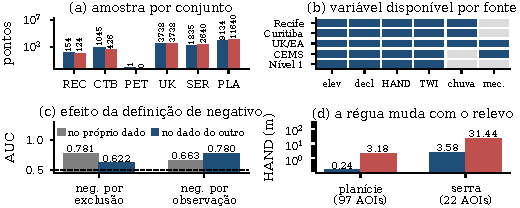
\includegraphics[width=0.97\columnwidth]{fig/fig2_datasets.pdf}
\caption{Conjuntos e desafios, com dados reais do projeto. (a) unidades por
conjunto, em log: o piloto UK-AOI é a primeira amostra pareada (3.738/3.738).
(b) HAND em Recife: as classes se sobrepõem. (c) coeficiente de Firth da chuva em
Curitiba: forte em 2023--2025 e nulo em 2026. (d) a mesma quebra no
\emph{walk-forward}.}
\label{fig:datasets}
\end{figure}

% ------------------------------ TABELA I ------------------------------
\begin{table*}[!t]
\caption{Resumo de materiais e métodos; a Seção~II contextualiza cada linha.}
\label{tab:mm}
\centering
\renewcommand{\arraystretch}{0.95}
\scriptsize
\begin{tabular}{@{}>{\raggedright\arraybackslash}p{2.05cm}>{\raggedright\arraybackslash}p{7.6cm}>{\raggedright\arraybackslash}p{6.5cm}@{}}
\toprule
\textbf{Materiais} & \textbf{Descrição} & \textbf{Observações} \\
\midrule
Rótulo &
Positivos: SEDEC/Recife (154), SIAC 156/Curitiba (1.045), Diário Oficial,
ANA/SNIRH, Global Flood Database~\cite{tellman2021}. \textbf{Negativos
observados}: Environment Agency/UK (31.672 \emph{outlines}; 262 eventos no
piloto) e Copernicus EMS EMSR720 (216,55\,km$^2$; 5,94:1) &
Registro de ausência, não ausência de registro; o tipo de evento separa
inundação de movimento de massa na origem. \\

Bases, variáveis e modelos &
MDT PE3D 10\,m e SGB/CPRM; CHIRPS~\cite{funk2015} e ERA5-Land~\cite{munoz2021};
Sentinel-1/2, MapBiomas e WorldCover (auxiliares). Elevação, declividade,
HAND~\cite{renno2008} e TWI~\cite{beven1979} por D-infinity, decaimento e pico de
chuva. Firth~\cite{firth1993} como rota primária e GBM/GAM/EBM como diagnóstico;
\emph{gate} EPV~\cite{peduzzi1996}, \emph{bootstrap} $N$\,=\,1000, blocos
espaciais, grupos por evento e \emph{walk-forward} &
Nenhuma variável derivada do rótulo, de escore ou de limiar; as orbitais
\textbf{não são causais}. A rota primária segue linear mesmo quando o não linear
tem AUC maior. \\

Produto, ambiente e recursos &
API FastAPI com contrato de inferência e geoprocessamento sob demanda;
\emph{model card}~\cite{mitchell2019}; camada LLM. Python 3.10 com
\texttt{firthlogist}, \texttt{scikit-learn}, \texttt{interpret},
\texttt{rasterio}/GDAL, \texttt{whitebox} e \texttt{pytest}; estação de 10 núcleos
e 15,5\,GB, sem GPU; QGIS 3, GEE, Git &
A LLM lê o \emph{payload} já decidido. Recursos suficientes e medidos: Firth
0,056\,s e EBM 25,3\,s. \\
\bottomrule
\end{tabular}
\end{table*}

% =====================================================================
\section{Etapas do Projeto e Marcos Físicos}
\label{sec:etapas}

\textbf{E0 e E1 --- Base consolidada e escopo congelado (concluídas).} Corpus,
governança de \emph{claims}, Protocolo C e o teste de ablação que mediu o
\emph{proxy learning}; em seguida, a definição escrita de qual documento rege o
trabalho. \emph{Evidência}: artefatos versionados, os três valores de acurácia
balanceada e uma afirmação de estado por arquivo.

\textbf{E2 --- Fechamento do negativo observado (M1).} Extrair as variáveis de
chuva sobre a amostra pareada do piloto inglês e aplicar o critério de separação
de mecanismo aos registros brasileiros. \emph{Entregável}: conjunto de treino com
negativo adjudicado. \emph{Evidência}: contagem por classe e por grupo de
validação, com os quatro critérios documentados.

\textbf{E3 --- Validação prospectiva sobre o novo conjunto (M2).} Ajustar o
modelo e submetê-lo a \emph{walk-forward} e blocos espaciais. \emph{Entregável}:
tabelas de coeficientes com intervalo e de desempenho por corte.
\emph{Evidência}: nenhum ajuste feito depois de olhar o teste, e o piso de
eventos por preditor verificado antes de cada ajuste.

\textbf{E4 --- Encerramento da série de não linearidade (M3).} A série está
saturada: confirmou não linearidade real, mas nenhuma rodada resolveu a quebra de
2026 da Fig.~\ref{fig:datasets}(c--d). \emph{Entregável}: nota de encerramento
declarando a rota primária linear. \emph{Evidência}: nenhuma rodada nova após o
marco.

\textbf{E5 --- Camada de explicação sobre o contrato (M4).} Implementar e testar
a LLM sobre respostas reais da API, inclusive as de recusa. \emph{Entregável}:
cenários com resposta estruturada e explicação correspondente. \emph{Evidência}:
nenhuma explicação contradiz o \emph{payload} nem preenche escore ausente.

\textbf{E6 e E7 --- Congelamento, redação e pôster (M5--M7).} Testes completos,
repositório limpo e \emph{tag} de congelamento; depois dessa data admite-se
apenas redação, sobre os artefatos congelados. \emph{Evidência}: cada número do
manuscrito rastreável a um arquivo.

\textbf{Riscos e revisão do plano.} Três etapas têm risco identificado e rota
alternativa declarada agora, não improvisada depois. Em E2, a paridade de fonte
de chuva entre Brasil e Inglaterra pode não ser alcançável; então o piloto inglês
vira conjunto de sensibilidade, não de treino conjunto. Em E3, o desempenho prospectivo pode não superar o acaso; o
resultado é publicado como está, com a discussão deslocada para as condições em
que o rótulo administrativo perde validade. Em E5, se a explicação divergir do \emph{payload} em algum cenário, a
camada é reduzida a um gerador de texto por regras sobre os mesmos campos.
Nenhuma dessas rotas altera a pergunta de pesquisa.

% =====================================================================
\section{Cronograma}
\label{sec:crono}

O cronograma (Tabela~\ref{tab:crono}) cobre da submissão deste plano à
apresentação final e incorpora os \emph{checkpoints} da disciplina: Entrega 01
(29/08), Entrega 02 (31/10), Entrega 03 (09/11) e a sessão de pôsteres (17/11).
O estado da arte já está em curso e sustenta este documento, permanecendo ativo
até a redação. Como o trabalho é individual, as etapas não correm em paralelo
entre pessoas, mas se sobrepõem no tempo: a análise acompanha a experimentação e
a redação começa antes do congelamento. As etapas foram identificadas de antemão
sem que a ordem de conclusão seja obrigatória, e a distribuição prevê folga
porque pesquisa costuma exceder o prazo estimado. Os intervalos de 08/09 e 13/10
seguem sem tarefa nova; 24/11 e 01/12 são contingência.

\begin{table}[!h]
\caption{Cronograma (quinzenas). E01 29/08, E02 31/10, E03 09/11, defesa 17/11.}
\label{tab:crono}
\centering
\renewcommand{\arraystretch}{1.0}
\setlength{\tabcolsep}{2.6pt}
\scriptsize
\begin{tabular}{@{}>{\raggedright\arraybackslash}p{1.95cm}ccccccc@{}}
\toprule
\textbf{Atividade} & \textbf{09--29} & \textbf{01--15} & \textbf{16--29} &
\textbf{30/09--} & \textbf{14--31} & \textbf{01--09} & \textbf{10--17} \\
 & \textbf{ago} & \textbf{set} & \textbf{set} & \textbf{13/10} &
\textbf{out} & \textbf{nov} & \textbf{nov} \\
\midrule
Estado da arte          & X & X & X &   &   &   &   \\
Dados (E2)              & X & X &   &   &   &   &   \\
Experimentação (E3--E4) &   & X & X &   &   &   &   \\
Produto/LLM (E5)        &   &   & X & X &   &   &   \\
Análise                 &   &   & X & X & X &   &   \\
Auditoria (E6)          &   &   &   & X &   &   &   \\
Redação (E7)            &   &   &   & X & X & X &   \\
Pôster e defesa         &   &   &   &   &   & X & X \\
\midrule
\textit{Checkpoints} & \textbf{E01} & & & & \textbf{E02} & \textbf{E03} & \textbf{Def.} \\
\bottomrule
\end{tabular}
\end{table}

% =====================================================================
\fontsize{6.8}{7.4}\selectfont
\begin{thebibliography}{99}
\setlength{\itemsep}{0.4pt}
\setlength{\parskip}{0pt}


\bibitem{tellman2021}
B. Tellman \emph{et al.}, ``Satellite imaging reveals increased proportion of
population exposed to floods,'' \emph{Nature}, vol. 596, pp. 80--86, 2021.

\bibitem{renno2008}
C. D. Rennó \emph{et al.}, ``HAND, a new terrain descriptor using SRTM-DEM:
Mapping terra-firme rainforest environments in Amazonia,''
\emph{Remote Sensing of Environment}, vol. 112, no. 9, pp. 3469--3481, 2008.


\bibitem{beven1979}
K. J. Beven and M. J. Kirkby, ``A physically based, variable contributing area
model of basin hydrology,'' \emph{Hydrological Sciences Bulletin}, vol. 24,
no. 1, pp. 43--69, 1979.


\bibitem{li2022pul}
W. Li \emph{et al.}, ``A positive-unlabeled learning algorithm for urban flood
susceptibility modeling,'' \emph{Land},
vol. 11, no. 11, art. 1971, 2022.


\bibitem{agostini2024}
G. Agostini, E. Pierson, and N. Garg, ``A Bayesian spatial model to correct
under-reporting in urban crowdsourcing,'' in \emph{Proc. AAAI}, vol. 38, 2024,
pp. 21\,888--21\,896.

\bibitem{firth1993}
D. Firth, ``Bias reduction of maximum likelihood estimates,''
\emph{Biometrika}, vol. 80, no. 1, pp. 27--38, 1993.


\bibitem{peduzzi1996}
P. Peduzzi \emph{et al.}, ``A simulation study of the number of events per
variable in logistic regression analysis,'' \emph{J. Clin. Epidemiol.}, vol. 49,
no. 12, pp. 1373--1379, 1996.


\bibitem{funk2015}
C. Funk \emph{et al.}, ``The climate hazards infrared precipitation with
stations,'' \emph{Scientific Data}, vol. 2, art. 150066, 2015.

\bibitem{munoz2021}
J. Muñoz-Sabater \emph{et al.}, ``ERA5-Land: a global reanalysis dataset for land
applications,'' \emph{Earth Syst. Sci. Data}, vol. 13, pp. 4349--4383, 2021.

\bibitem{mitchell2019}
M. Mitchell \emph{et al.}, ``Model cards for model reporting,'' \emph{Proc. ACM
FAT*}, pp. 220--229, 2019.

\end{thebibliography}

\end{document}

